\documentclass[../Results.tex]{subfiles}

\begin{document}
	\begin{figure*}
		\centering
		\subfloat[contour]{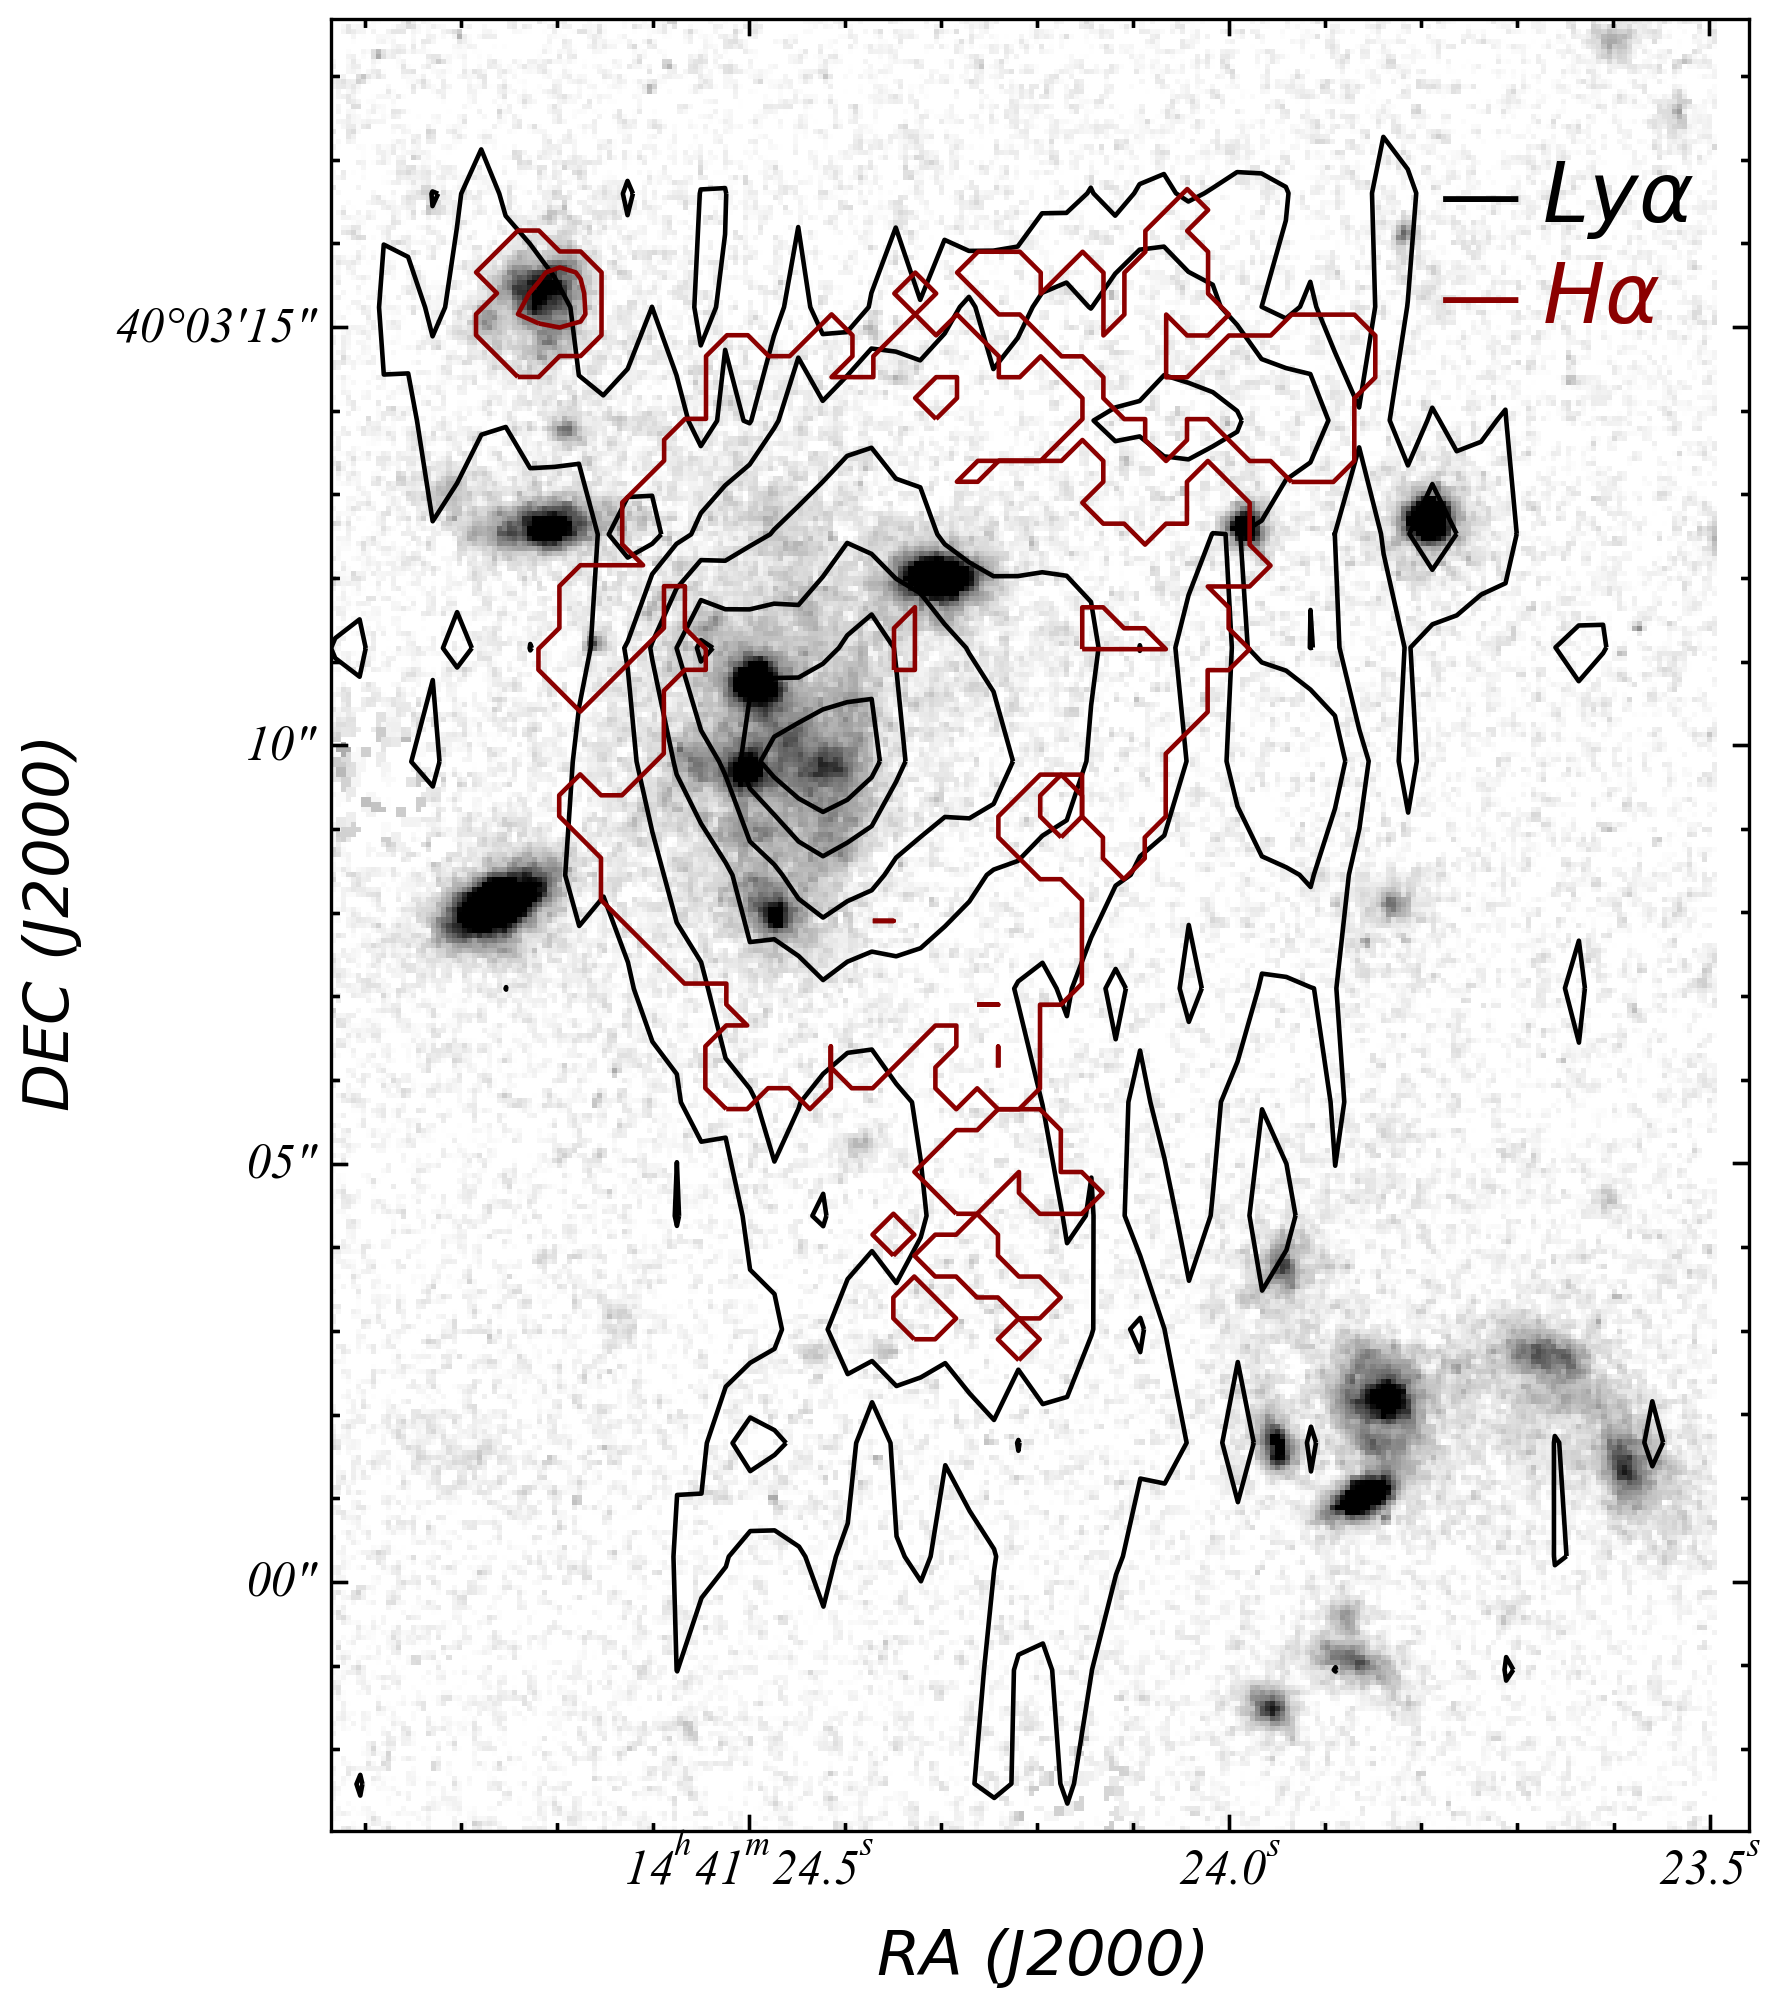
\includegraphics[width=0.5\textwidth]{figs/raito_contour}}
		\subfloat[ratio]{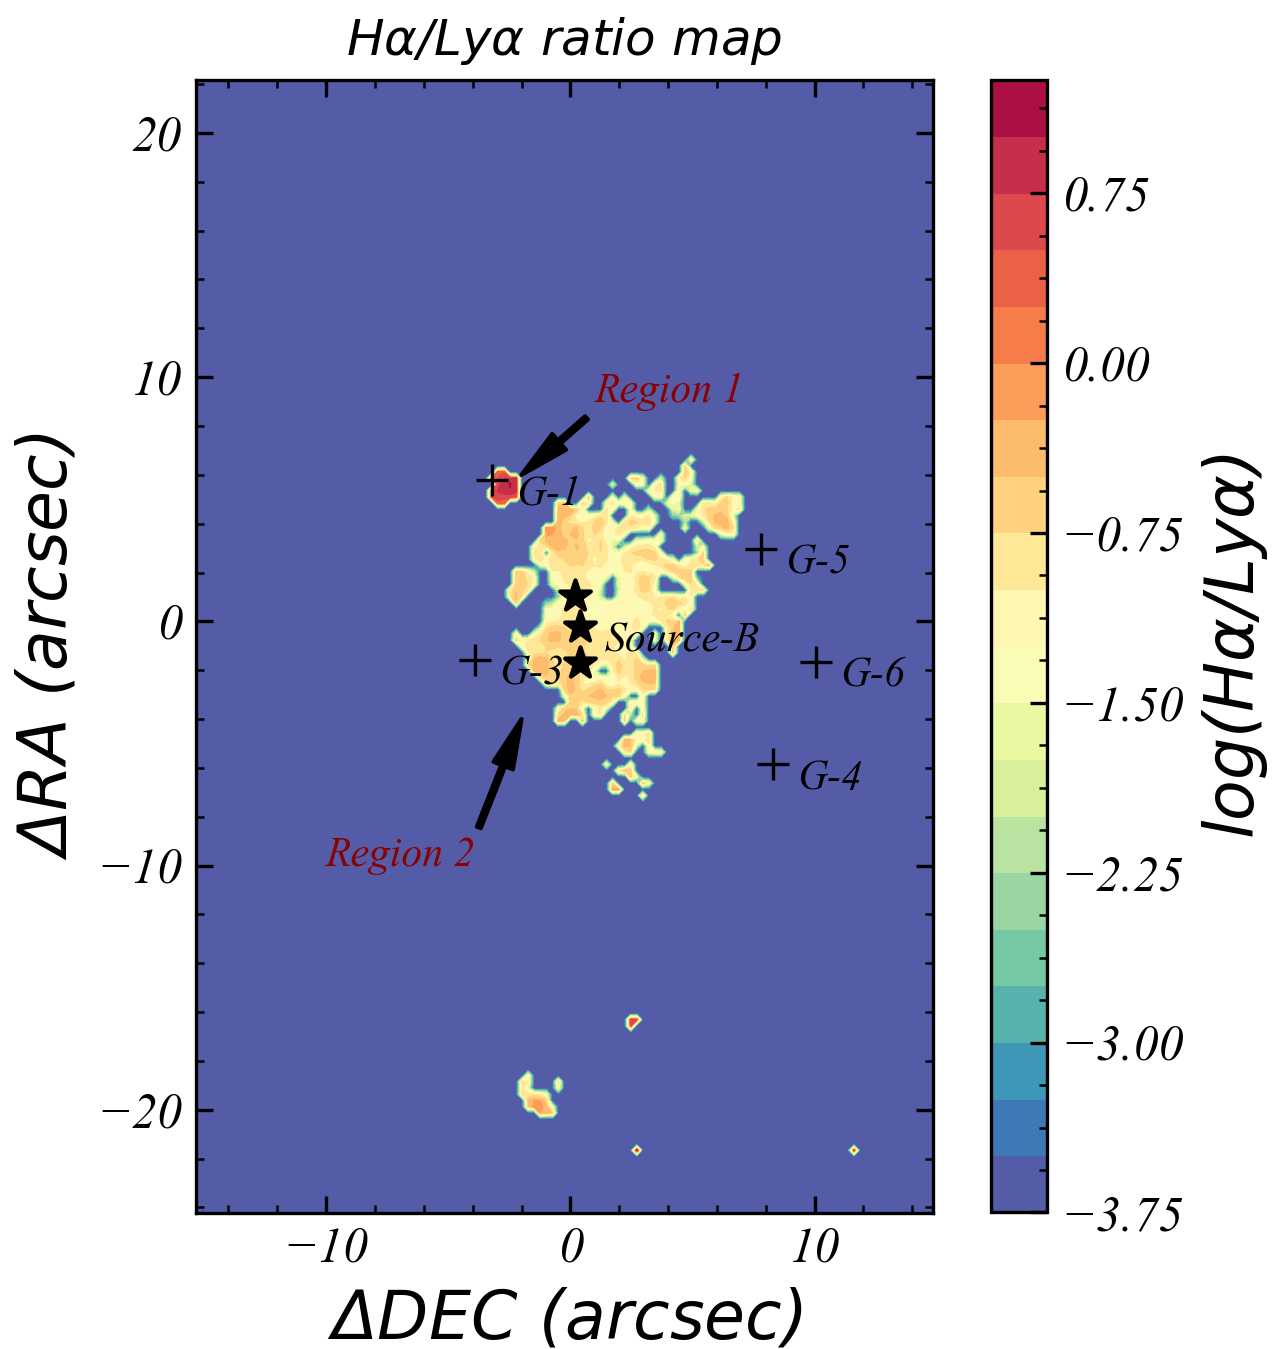
\includegraphics[width=0.5\textwidth]{figs/H_alpha_ly_alpha_ratio}}
		\label{H_alpha}
		\caption{Left: HST image of MAMMOTH-1 from circle 24,25, PI: Cai. We overlay on it Ly$\alpha$ HeII and CIV psudo narrow band images. Black contour is Ly$\rm \alpha$, blue contour is HeII, green contour is CIV. We also mark source-B with red mark and sources at the same redshift with yellow mark. We also plot circle with raidus of 1$\rm arcsec^{2}$. Right: spectra of the 3 emission lines extracted from aperture center on source-B with radius 1$\rm arcsec^{2}$, we fit them with one-component gaussian function.}
	\end{figure*}
\end{document}